\documentclass[]{article}

\usepackage{tikz}
\usepackage{amsmath}
\usepackage{amsfonts}
\usepackage{amssymb}
\usepackage{tkz-base}
\usepackage{tkz-euclide}
\usepackage{xcolor}
\usepackage{pgfplots}

% Required package
\usetikzlibrary{positioning}
\usetikzlibrary{svg.path}
\usetikzlibrary{arrows}
\usetikzlibrary{shapes.geometric,calc}

\newdimen\XCoord
\newdimen\YCoord
\newcommand*{\ExtractCoordinate}[1]{\path (#1); \pgfgetlastxy{\XCoord}{\YCoord};}%

%opening
\title{Joint--Based Linear Control}
\author{Glen Henshaw\\Craig Carignan}

\begin{document}

\maketitle


\section{Intro}
Here's a block diagram of our robotic system:
\begin{figure}[h!]
 \centering
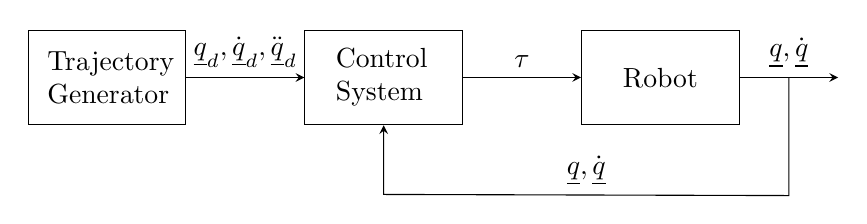
\begin{tikzpicture}
 % Sum shape
 \node[draw, 
        minimum width=2cm,
        minimum height=1.2cm
        ] (trajgen) at (0,0){\parbox[t]{0.125\linewidth}{Trajectory\\Generator}};

% Controller
\node [draw,
    minimum width=2cm,
    minimum height=1.2cm,
    right=1.5cm of trajgen
]  (controller) {\parbox[t]{0.1\linewidth}{Control\\System}};
 
% System H(s)
\node [draw,
    minimum width=2cm, 
    minimum height=1.2cm,
    right=1.5cm of controller
] (system) {Robot};
  
% Arrows with text label
%\draw[-stealth] (trajgen.north east) -- (controller.north west)
%    node[midway,above]{$\Omega$};
\draw[-stealth] (trajgen.east) -- (controller.west)
    node[midway,above]{$\underline{q}_{d}, \dot{\underline{q}}_{d}, \ddot{\underline{q}}_{d}$};
%\draw[-stealth] (trajgen.south east) -- (controller.south west)
%    node[midway,above]{$\ddot{\Omega}$};
 
\draw[-stealth] (controller.east) -- (system.west) 
    node[midway,above]{$\tau$};

\draw[-stealth] (system.east) -- ++ (1.25,0) 
    node[midway](output){}node[midway,above]{$\underline{q}, \dot{\underline{q}}$};

\ExtractCoordinate{controller.south}
\draw[-stealth] (output.center) -- ++ (0,-1.5) -- (\XCoord, \YCoord-25) node[midway,above]{$\underline{q}, \dot{\underline{q}}$} -- (controller.south);

%\draw[-stealth] (output.center) -- ++ (0,-2) -- (\XCoord-10, \YCoord-37) node[midway,above]{$\dot{q}$} -- (controller.south west);

  
\end{tikzpicture}
\end{figure}

And remember from last time that we can write the dynamics of our robot in the form
\begin{displaymath}
 \underline{\tau} = M(\underline{q}) \ddot{\underline{q}} +C(\underline{q}, \underline{\dot{q}})\dot{q} + E(\underline{q}, \underline{\dot{q}})
\end{displaymath}
We want to figure out the design of a ``control law'' -- an equation for $\underline{\tau}$ that causes the robot to track the desired trajectory $\underline{q}_{d}, \dot{\underline{q}}_{d}, \ddot{\underline{q}}_{d}$. The problem is that the robot dynamics are pretty complicated. Ideally, we could use an ``open loop controller'' of the form
\begin{displaymath}
 \underline{\tau} = M(\underline{q}_{d}) \ddot{\underline{q}}_{d} +C(\underline{q}_{d}, \underline{\dot{q}}_{d})\dot{q}_{d} + E(\underline{q}_{d}, \underline{\dot{q}}_{d})
\end{displaymath}
but in practice this doesn't work very well because we don't know $M$, $C$, or $E$ exactly, and plus there are always unmodelled dynamics present --  we've treated our robot as if it is completely rigid, which it isn't, we've neglected the dynamics of the gears and motors in the actuator, there are always air currents or (in the SSL) water effects, and the occasional human who wanders through our robot's workspace and pushes on it.

In general, control systems make use of the actual trajectory to compute the input torques, This is known as ``closed--loop'' control.
\begin{eqnarray}
 \underline{\tilde{q}} & = & \underline{q}_{d} - \underline{q} \nonumber\\
 \underline{\dot{\tilde{q}}} & = & \dot{\underline{q}}_{d} - \dot{\underline{q}} \nonumber
\end{eqnarray}
$(\underline{\tilde{q}}, \dot{\tilde{\underline{q}}})$ is called ``servo error''. The controller computes the torque based on servo error. Linear controllers use linear combinations of the servo errors.

There are several performance criteria we want out of controllers:
\begin{itemize}
 \item stability (the requirement that the errors be bounded as long as the disturbances are bounded)
 \item bandwidth (the ability of the robot to quickly track rapidly changing desired trajectories)
 \item damping (no oscillations in the output -- we'll talk about this in a minute)
\end{itemize}

The easiest and most common approach to controlling robot arms is INDEPENDENT JOINT CONTROL, where we assume that each joint of the arm is dynamically independent of all the others, e.g that the dynamics really look like
\begin{equation}
 \tau_{i} = m_{i}\ddot{q}_{i} + b_{i}\dot{q}_{i}+e_{i}(q{i}) \label{SMD}
\end{equation}
Notice that this looks like the dynamics of a simple spring--mass--damper system:

\begin{figure}[h!]
\centering
 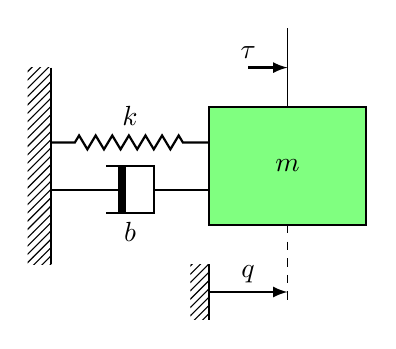
\begin{tikzpicture}[every node/.style={outer sep=0pt},thick,
 mass/.style={draw,thick},
 spring/.style={thick,decorate,decoration={zigzag,pre length=0.3cm,post
 length=0.3cm,segment length=6}},
 ground/.style={fill,pattern=north east lines,draw=none,minimum
 width=0.75cm,minimum height=0.3cm},
 dampic/.pic={\fill[white] (-0.1,-0.3) rectangle (0.3,0.3);
 \draw (-0.3,0.3) -| (0.3,-0.3) -- (-0.3,-0.3);
 \draw[line width=1mm] (-0.1,-0.3) -- (-0.1,0.3);}]

  \node[mass,minimum width=2cm,minimum height=1.5cm,fill=green!50] (m1) {$m$};
   \node[left=2cm of m1,ground,minimum width=3mm,minimum height=2.5cm] (g1){};
  \draw (g1.north east) -- (g1.south east);

  \draw[spring] ([yshift=3mm]g1.east) coordinate(aux)
   -- (m1.west|-aux) node[midway,above=1mm]{$k$};

  \draw ([yshift=-3mm]g1.east) coordinate(aux')
   -- (m1.west|-aux') pic[midway]{dampic} node[midway,below=3mm]{$b$};
 
  \foreach \X in {1}  
  {\draw[thin] (m\X.north) -- ++ (0,1) coordinate[midway](aux\X);
   \draw[latex-] (aux\X) -- ++ (-0.5,0) node[above]{$\tau$}; 
   \draw[thin,dashed] (m\X.south) -- ++ (0,-1) coordinate[pos=0.85](aux'\X);
   \draw[latex-] (aux'\X) -- ++ (-1,0) node[midway,above]{$q$}
    node[left,ground,minimum height=7mm,minimum width=1mm] (g'\X){};
   \draw[thick] (g'\X.north east) -- (g'\X.south east);
  }

\end{tikzpicture}
\end{figure}
...only with no spring term in the dynamics. So, really a mass--damper system with some environmental terms. So what if we design a controller that explicitly turns this into a spring--mass--damper system? In that case we want dynamics that look something like:
\begin{displaymath}
 \tau = m\ddot{q} + b\dot{q}+kq
\end{displaymath}
One way to approximate this is to design a controller that does the following:
\begin{displaymath}
 \tau_{c} = - k_{v}\dot{q} - k_{p}(q-q_{d})
\end{displaymath}

So let's substitute this $\tau_{c}$ in for $\tau$ in Equation \ref{SMD}:
\begin{displaymath}
 m\ddot{q} + b\dot{q}+e(q) = - k_{v}\dot{q} - k_{p}(q_{d}-q)
\end{displaymath}
or
\begin{displaymath}
 m\ddot{q} + (b+k_{v})\dot{q} + k_{p}(q_{d}-q) + e(q, \dot{q}) = 0
\end{displaymath}
if we assume, for the moment, that $q_{d}=0$ and if we neglect $e$, we can see that this looks precisely like a spring--mass--damper system with a mass, damping constant, and spring stiffness that we have specified. Assuming all of these coefficients are positive, the system will have a stable equilibrium point at the origin.

A common way of writing this equation is the ``normal form'':
\begin{displaymath}
 \ddot{q} + \underbrace{\frac{b+k_{v}}{m}}_{2\zeta \omega_{n}}\dot{q} + \underbrace{\frac{k_{p}}{m}}_{\omega_{n}^{2}}q = 0
\end{displaymath}
where
\begin{eqnarray}
 \omega_{n} & = & \sqrt{\frac{k_{p}}{m}}\ \ \  \text{``natural frequency''} \nonumber \\
 \zeta & = & \frac{b+k_{v}}{2m\omega_{n}}\ \ \  \text{``damping ratio''} \nonumber
\end{eqnarray}
The ``unforced response'' of this system looks like:
\begin{figure}[h!]
 \centering
 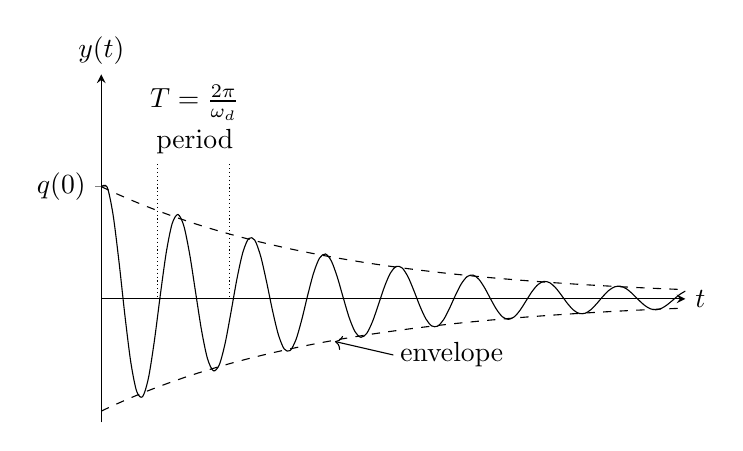
\begin{tikzpicture}
    \begin{axis}[
            width=9cm,
            height=6cm,
            axis lines=middle,
            xmin=0, xmax=50,
            ymin=-1.1, ymax=2,
            xlabel=$t$,
            ylabel={$y(t)$},
            xlabel style={at=(current axis.right of origin), anchor=west},
            ylabel style={at=(current axis.above origin), anchor=south},
            ytick={0, 1},
            yticklabels={$0$, $q(0)$},
            xtick={0},
            xticklabels={$0$}
        ]
        \draw[black, densely dotted] (axis cs:4.8,1.2) -- (axis cs:4.8,0);
        \draw[black, densely dotted] (axis cs:11,1.2) -- (axis cs:11,0);
        \draw (axis cs:8,1.4) node{period};
        \draw (axis cs:8, 1.75) node{$T=\frac{2\pi}{\omega_{d}}$};
        \draw (axis cs:30, -0.5) node{envelope};
        \draw[->] (axis cs:25,-0.5) -- (axis cs:20,-0.38);
        \addplot[smooth, 
                 black,
                 mark=none,
                 domain=0:50,
                 samples=100]
        {-(1-exp(-0.05*x)*(cos(deg(sqrt(1-0.05^2)*x))+0.3/(sqrt(1-0.05^2))*sin(deg(sqrt(1-0.05^2)*x))))+1};
        \addplot[smooth, 
            black,
            dashed,
            mark=none,
            domain=0:50,
            samples=100]
        {-(1-exp(-0.05*x))+1};
        \addplot[smooth, 
            black,
            dashed,
            mark=none,
            domain=0:50,
            samples=100]
        {(1-exp(-0.05*x))-1};

    \end{axis}

\end{tikzpicture}
\end{figure}

The envelope has the form
\begin{displaymath}
 e^{-\zeta\omega_{n}t}
\end{displaymath}
and $\omega_{d}$ is the ``damped natural frequency'',
\begin{displaymath}
 \omega_{d} = \sqrt{1-\zeta^{2}}\omega_{n}
\end{displaymath}

This is the step response:

\begin{figure}[h!]
 \centering
 \begin{tikzpicture}
    \begin{axis}[
            width=9cm,
            height=6cm,
            axis lines=middle,
            xmin=0, xmax=15,
            ymin=0, ymax=1.5,
            xlabel=$t$,
            ylabel={$y(t)$},
            xlabel style={at=(current axis.right of origin), anchor=west},
            ylabel style={at=(current axis.above origin), anchor=south},
            xtick={0, 01.96605, 3.2236, 11.0855},
            xticklabels={$0$, $$, $t_p$, $t_s$},
            every x tick/.style={black},
            ytick={0, 1, 1.3714},
            yticklabels={$0$, $1$, $M_p$},
            every y tick/.style={black}
        ]
       % \addplot[black, densely dotted] coordinates{(0.4726,0.1)} -- (axis cs:0,0.1);
       % \addplot[black, densely dotted] coordinates{(0.4726,0.1)} -- (axis cs:0.4726,0);
        %
      %  \addplot[black, densely dotted] coordinates{(1.79398,0.9)} -- (axis cs:0,0.9);
      %  \addplot[black, densely dotted] coordinates{(1.79398,0.9)} -- (axis cs:1.79398,0);
        %
        \addplot[black, densely dotted] coordinates{(1.96605,1)} -- (axis cs:1.96605,0);
        %
      %  \addplot[black, densely dotted] coordinates{(3.2236,1.3714)} -- (axis cs:0,1.3714);
        \addplot[black, densely dotted] coordinates{(3.2236,1.3714)} -- (axis cs:3.2236,0);
        %
        \addplot[black, densely dotted] coordinates{(11.0855,1.025)} -- (axis cs:11.0855,0);

        \addplot[black, dashed] coordinates{(15,1)} -- (axis cs:0,1);
        %
        \addplot[cyan, dashed] coordinates{(15,0.975)} -- (axis cs:10,0.975);
        \addplot[cyan, dashed] coordinates{(15,1.025)} -- (axis cs:10,1.025);
        %
        \addplot[smooth, 
                 black,
                 thick,
                 mark=none,
                 domain=0:12.4,
                 samples=100]
        {1-exp(-0.3*x)*(cos(deg(sqrt(1-0.3^2)*x))+0.3/(sqrt(1-0.3^2))*sin(deg(sqrt(1-0.3^2)*x)))};
        %
        \addplot[black, thick] coordinates{(15,0.9872)} -- (axis cs:12.4,0.9872);
        %
        \coordinate (trleft) at (axis cs:0,0);
        \coordinate (trright) at (axis cs:1.96605,0);
        %
        \coordinate (tr1left) at (axis cs:0.4726,0);
        \coordinate (tr1right) at (axis cs:1.79398,0);
        %
        \coordinate (ess1) at (axis cs:14,1.1);
        \coordinate (ess2) at (axis cs:14,1);
        \coordinate (ess3) at (axis cs:14,0.9872);
        \coordinate (ess4) at (axis cs:14,0.8872);
    \end{axis}

%    \draw [densely dotted] (tr1left) -- ++(0,-0.5cm) coordinate (a1);
%    \draw [densely dotted](tr1right) -- ++(0,-0.5cm) coordinate (a2);
%    \draw [<->] ([yshift=2pt]a1) -- ([yshift=2pt]a2) node [midway,fill=white] {${\scriptstyle \hat{t}_r}$};

    \draw [densely dotted] (trleft) -- ++(0,-1cm) coordinate (b1);
    \draw [densely dotted](trright) -- ++(0,-1cm) coordinate (b2);
    \draw [<->] ([yshift=2pt]b1) -- ([yshift=2pt]b2) node [midway,fill=white] {$t_r$};

    \draw [->] (ess1) node [right] {$\bar{\epsilon}$} -- (ess2);
    \draw [<-] (ess3) -- (ess4);

\end{tikzpicture}
\end{figure}

where:
\begin{eqnarray}
    & M_{p} = e^{\frac{-\zeta\omega_{n}}{\omega_{d}}}\pi \times 100\% & \ \ \ \text{``Peak Overshoot''} \nonumber\\
    & t_{p} = \frac{\pi}{\omega_{d}} & \ \ \ \text{``Peak time (1/2 period)''} \nonumber \\
    & t_{r} = \frac{1}{\omega_{d}}\tan^{-1}\left(\frac{\omega_{d}}{\zeta\omega_{n}}\right) & \ \ \  \text{``rise time''}\nonumber \\
    & t_{s} = \frac{4}{\zeta\omega_{n}} & \ \ \ \text{``settling time (2\%)''} \nonumber
\end{eqnarray}

\section{Solving 2nd--Order Differential Equations Via the LaPlace Transform}
We can transform an ODE into an algebraic equation via the Laplace Transform:
\begin{displaymath}
 \mathcal{L}\left\{\ddot{x}+2\zeta\omega_{n}\dot{x} + \omega_{n}^{2}x=0\right\}
\end{displaymath}
\begin{displaymath}
 s^{2}X(s)+2\zeta\omega_{n}sX(s)+\omega_{n}^{2}X(s)=0
\end{displaymath}
\begin{displaymath}
 \underbrace{\left(s^{2}+2\zeta\omega_{n}s+\omega_{n}^{2}\right)}_{\text{``characteristic equation''}}X(s)=0
\end{displaymath}
The roots of the characteristic equation:
\begin{enumerate}
 \item $\zeta>1$ (overdamped)
 \begin{displaymath}
  s_{1,2} = -\zeta\omega_{n} \pm \sqrt{\zeta^{2}-1}\omega_{n} \Rightarrow x(t) = c_{1}e^{s_{1}t} + c_{2}e^{s_{2}t}
 \end{displaymath}
This is a pure decaying exponential:

\begin{tikzpicture}
    \begin{axis}[
            width=9cm,
            height=6cm,
            axis lines=middle,
            xmin=0, xmax=50,
            ymin=-0.1, ymax=1,
            xlabel=$t$,
            ylabel={$y(t)$},
            xlabel style={at=(current axis.right of origin), anchor=west},
            ylabel style={at=(current axis.above origin), anchor=south},
            ytick={0, 1},
            yticklabels={$0$, $q(0)$},
            xtick={0},
            xticklabels={$0$}
        ]
        \addplot[smooth, 
            black,
            dashed,
            mark=none,
            domain=0:50,
            samples=100]
        {-(1-exp(-0.05*x))+1};

    \end{axis}

\end{tikzpicture}

\item $\zeta<1$ (underdamped)
\begin{displaymath}
 s_{1,2} = -\zeta\omega_{n}\pm\sqrt{1-\zeta^{2}}\omega_{n}j \Rightarrow x(t) = e^{-\zeta\omega_{n}t}\left(c_{1}\cos(\omega_{d}t) + c_{2}\sin(\omega_{d}t)\right)
\end{displaymath}
where $j=\sqrt{-1}$ and $\omega_{d}=\sqrt{1-\zeta^{2}}\omega_{n}$
or
\begin{displaymath}
x(t) = r\ e^{-\zeta\omega_{n}t}\cos(\omega_{d}t - \underbrace{\delta}_{\text{phase}})
\end{displaymath}
where
\begin{eqnarray}
 r & = & \sqrt{c_{1}^{2}+c_{2}^{2}} \nonumber \\
 \delta & = & \text{atan2}(c_{2},c_{1}) \nonumber
\end{eqnarray}
This is (hopefully!) decaying but oscillatory:

\begin{tikzpicture}
    \begin{axis}[
            width=9cm,
            height=6cm,
            axis lines=middle,
            xmin=0, xmax=20,
            ymin=-0.75, ymax=1,
            xlabel=$t$,
            ylabel={$y(t)$},
            xlabel style={at=(current axis.right of origin), anchor=west},
            ylabel style={at=(current axis.above origin), anchor=south},
            ytick={0, 1},
            yticklabels={$0$, $q(0)$},
            xtick={0},
            xticklabels={$0$}
        ]
        \addplot[smooth, 
            black,
            dashed,
            mark=none,
            domain=0:50,
            samples=100]
{-(1-exp(-0.2*x)*(cos(deg(sqrt(1-0.2^2)*x))+0.3/(sqrt(1-0.2^2))*sin(deg(sqrt(1-0.2^2)*x))))+1};
    \end{axis}

\end{tikzpicture}
\end{enumerate}

\subsection{Example}
Assume we have a linear dynamic system
\begin{displaymath}
 m\ddot{x}+b\dot{x}+kx=f
\end{displaymath}
\begin{enumerate}
 \item Find $x(t)$ for the ICs $x(0)=-1$, $\dot{x}(0)=0$
 Characteristic equation:
 \begin{displaymath}
s^{2}+\underbrace{1\cdot s}_{2\zeta\omega_{n}} + \underbrace{1}_{\omega_{n}^{2}} = 0
 \end{displaymath}
\begin{eqnarray}
 \Rightarrow \omega_{n}^{2} = 1 & \rightarrow & \omega_{n}=1 \nonumber \\
 2\zeta\omega_{n} = 1 & \rightarrow & \zeta=0.5 \nonumber
\end{eqnarray}
so the time solution is
\begin{displaymath}
 x(t) = e^{-\zeta\omega_{n}t}\left(c_{1}\cos(\omega_{d}T) + c_{2}\sin(\omega_{d}t)\right)
\end{displaymath}
where $\omega_{d}=\omega_{n}\sqrt{1-\zeta^{2}} = \sqrt{1-(0.5)^{2}} = \sqrt{3}/2$.

Apply the ICs to find $c_{1}$ and $c_{2}$:
\begin{eqnarray}
 x(0) & = & c_{1} = -1\ \ \ \Rightarrow c_{1}=-1 \nonumber  \\
 \dot{x}(0) & = & \omega_{d}c_{2}-\zeta\omega_{n}c_{1} = 0 \ \ \ \Rightarrow c_{2}=-1/\sqrt{3} \nonumber
\end{eqnarray}
so
\begin{displaymath}
 x(t) = e^{-1/2\ t}\left[\cos(\frac{\sqrt{3}}{2}t - \frac{1}{\sqrt{3}}\sin{\frac{\sqrt{3}}{2}t}\right]
\end{displaymath}
or
\begin{eqnarray}
 r & = & \sqrt{(-1)^{2}+(\frac{-1}{\sqrt{3}})^{2}} = \frac{2}{\sqrt{3}} \nonumber \\
 \delta & = & \text{atan2}\left(-1, -\frac{1}{\sqrt{3}}\right) = 120^{\circ} \nonumber
\end{eqnarray}

\item Now apply the P.D. controller
\begin{displaymath}
 f_{c} = -k_{p}x-k_{v}\dot{x}
\end{displaymath}
what gains do we need to achieve critical damping and stiffness=16?
\begin{eqnarray}
 \text{Dynamics:} && f = m\ddot{x}+b\dot{x}+kv \nonumber \\
 \text{Control:} && f_{c} = -k_{p}x - k_{v}\dot{x} \nonumber
\end{eqnarray}
The closed--loop dynamics are
\begin{eqnarray}
 m\ddot{x}+b\dot{x}+kx & = & -k_{p}x-k_{v}\dot{x} \nonumber \\
 m\ddot{x} + (b+k_{v})\dot{x} + (k+k_{p})x & = & 0 \nonumber
\end{eqnarray}
To find the stiffness:
\begin{eqnarray}
k_{total} & = & k+k_{p} \nonumber \\
16 & = & 1 + k_{p} \nonumber \\
\Rightarrow k_{p} & = & 15 \nonumber
\end{eqnarray}
to find the damping ($\zeta=1$):
\begin{eqnarray}
 2\zeta\omega_{n} & = & \frac{b+k_{v}}{m} \Rightarrow k_{v} = \underbrace{2\zeta}_{1}\underbrace{\omega_{n}}_{?}\underbrace{m}_{1} - \underbrace{b}_{1} \nonumber \\
 \omega_{n}^{2} & = & \frac{k+k_{p}}{m} = \frac{1+15}{1}=16\Rightarrow \omega_{n}=4 \nonumber \\
 \Rightarrow k_{v} & = & 2(1)(4)(1)-1 \nonumber \\
 \Rightarrow k_{v} & = & 7 \nonumber 
\end{eqnarray}


\end{enumerate}


\end{document}
